\section{Data Set}
\label{sec:dataset}
%本实验的数据集由小组成员采集于工业和信息化部电子第五研究所,采集对象包括六种不同的电子元器件,记录持续时间内测试电子元件的电流大小与时间。本实验的训练集为所采集的四号电子原件,包含1058条数据。其他数据集用于测试和验证,由于最后所预测的是以天数为单位的电子元件寿命而原始数据集在一天内多次测量电流,因此所有用于测试的数据集按照日期进行划分。
%其中每一天的电流值取该天多次测量的平均值。经过处理后所得数据集其中三号电子元件包括持续138天内的电流大小,
%五号电子元件包括持续的139天内电流大小,
%六号电子元件包括持续128天内电流的大小,
%七号电子元件包括持续139天内的电流大小,
%八号电子元件包括持续109天内的电流大小。
\section{Dataset Description}

The dataset for this experiment was collected by our team at the Fifth Research Institute of the Ministry of Industry and Information Technology. It includes six different types of electronic components, with recorded data capturing the current size and time over a continuous testing period. The training set consists of data from Component 4, containing 1,058 data points. Other datasets are used for testing and validation.

Since the final prediction targets the lifespan of electronic components in days, and the original dataset contains multiple current measurements within a single day, the data used for testing is divided by date. For each day, the current value is calculated as the average of all measurements taken on that day. After processing, the datasets for the components are as follows:
\begin{itemize}
    \item Component 3: Current measurements over 138 days.
    \item Component 5: Current measurements over 139 days.
    \item Component 6: Current measurements over 128 days.
    \item Component 7: Current measurements over 139 days.
    \item Component 8: Current measurements over 109 days.
\end{itemize}

This data processing approach ensures that the datasets are structured appropriately for analyzing the lifespan of the components.

\begin{figure}[H]
  \centering
     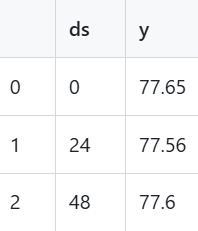
\includegraphics[scale=0.6]{figures/No.4data} % 替换为你的图片文件名
   %\includegraphics[width=0.8\linewidth]{egfigure.eps}

   \caption{No4.Data.
  ds represents the time interval in hours and y represents the current.}
   \label{fig:onecol}
\end{figure}

\begin{figure}[H]
  \centering
     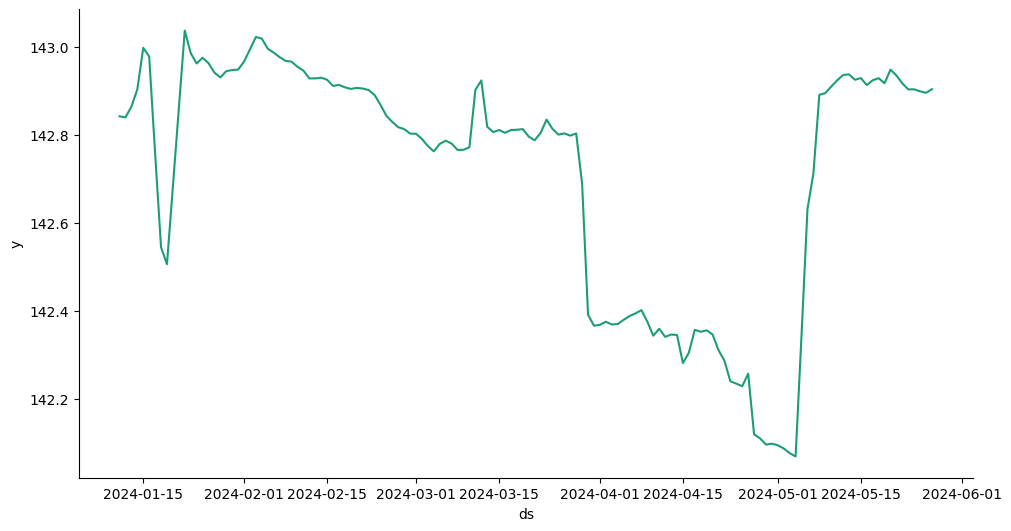
\includegraphics[width=\linewidth]{figures/No.3data} % 替换为你的图片文件名
   %\includegraphics[width=0.8\linewidth]{egfigure.eps}

   \caption{Visualization of Data for Component No. 3.
  ds represents the date and y represents the current.}
   \label{fig:onecol}
\end{figure}
